\chapter{The quasi-local approach: trapping horizons}
\label{s:loc}

\minitoc

\section{Introduction}

This chapter is in a draft stage.

\section{Trapped surfaces and singularity theorems}

\subsection{Trapped surfaces}

The concept of trapped surfaces has been introduced in Sec.~\ref{s:neh:trapped_surfaces}
(see in particular Fig.~\ref{f:neh:trapped_surf}). Let us recall that
a submanifold $\Sp$ of a $n$-dimensional spacetime ($n\ge 3$) is
a \defin{trapped surface}\index{trapped!surface} iff (i) $\Sp$ is a compact $(n-2)$-dimensional manifold
(without boundary), (ii) $\Sp$ is spacelike (positive definite induced metric)
and the two systems of null geodesics emerging orthogonally from $\Sp$ towards the future
locally converge, i.e. they have negative expansions at $\Sp$:
$\theta_{(\wl)} < 0$ and $\theta_{(\w{k})} < 0$ [Eq.~(\ref{e:neh:def_trapped_surf})],
$\wl$ and $\w{k}$ being
future-directed vectors tangent to these geodesics.

\begin{remark}
Trapped surfaces are sometimes called
\emph{closed trapped surfaces}\index{closed!trapped surface}\index{trapped!surface!closed --} (e.g. \cite{Penro65,HawkiE73}),
to stress their closed manifold aspect (compact without boundary).
We follow here the textbooks \cite{MisneTW73,Wald84} and call them merely
\emph{trapped surfaces}.
\end{remark}

\begin{example}[trapped surfaces in Schwarzschild spacetime]
Let $(\M,\w{g})$ be the Schwarzschild spacetime as defined in Sec.~\ref{s:sch:time_orientation} [Eq.~(\ref{s:sch:def_Schwarz_spacetime})]; it is entirely covered by the ingoing Eddington-Finkelstein coordinates
$(\ti,r,\th,\ph)$. Let $\Sp$ be any surface $(\ti,r) = \mathrm{const}$.
$\Sp$ is diffeomorphic to $\mathbb{S}^2$ and thus compact.
Moreover, from Eq.~(\ref{e:sch:Schwarz_metric_EF}), the metric induced by $\w{g}$
on $\Sp$ is $\w{q} = r^2 (\D\th^2 + \sin^2\th\D\ph^2)$, which is clearly positive definite, so
that $\Sp$ is spacelike. One reads also on the expression of $\w{q}$
that the area of  $\Sp$ is simply $A = 4\pi r^2$ (i.e. $r$ is the areal radius, cf. Sec.~\ref{s:sch:static_spher}).
If $\Sp$ is located in the black hole interior, i.e. if $0<r < 2m$,
Property~\ref{p:sch:r_decreasing} implies that $A$ is decreasing along any future-directed null
geodesic. It follows that $\Sp$ is trapped. On the contrary, if located in the black hole exterior
($r> 2m$), $\Sp$ is untrapped. This can be checked on Fig.~\ref{f:sch:rad_null_geod_EF},
where it appears clearly that, in the region $r>2m$, $r$ is increasing along the outgoing radial null geodesics, which are normal to $\Sp$.
\end{example}

\begin{figure}
\centerline{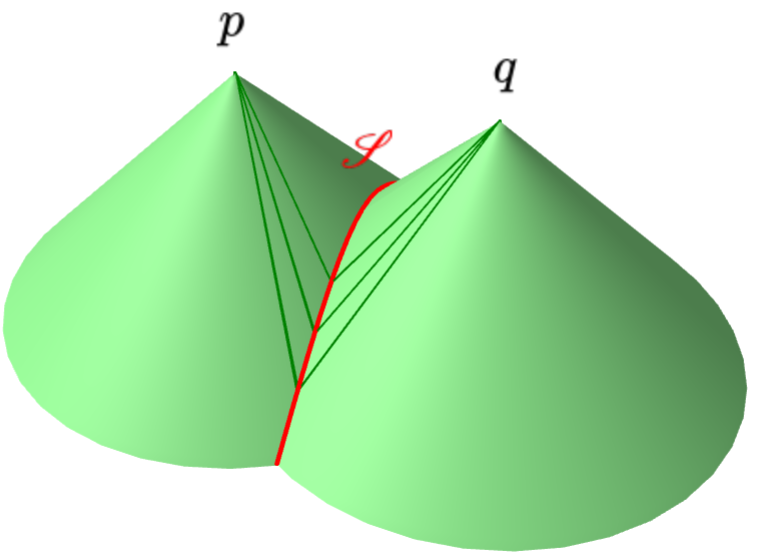
\includegraphics[width=0.6\textwidth]{loc_cone_intersect.png}}
\caption[]{\label{f:loc:cone_intersect} \footnotesize
Intersection $\Sp$ (red curve) of the past light cones of two points $p$ and $q$ in Minkowski spacetime.
Some light rays emerging from $\Sp$ in the two orthogonal null directions are depicted; the two sets
of light rays are both converging. Yet $\Sp$ is not trapped because it is not compact.
\textsl{[Figure generated by the notebook \ref{s:sam:loc_cone_intersect}]}
}
\end{figure}

The existence of a trapped surface is a characterization of
strong gravity\index{gravity!strong --}. More precisely it indicates that gravity is strong enough
to focus all light rays emitted from the surface.
This characterization is \emph{quasi-local}\index{quasi-local}, in the sense that it involves a \emph{surface}. The
surface can be ``small'' but it cannot be reduced to a point, to which the qualifier \emph{local}
would apply. Note that the hypothesis of \emph{compact} manifold is crucial in the definition of a
trapped surface. Without it, trapped surfaces would exist in Minkowski
spacetime, as the following example shows.

\begin{example}[a counter-example in Minkowkski spacetime]
Let us consider the intersection $\Sp$ of the past light cones $\mathscr{C}_p$ and $\mathscr{C}_q$
of two points $p$ and $q$ of Minkowski spacetime (cf. Fig.~\ref{f:loc:cone_intersect}).
Being a cross-section of the null hypersurface $\mathscr{C}_p$ (or $\mathscr{C}_q$),
$\Sp$ is a spacelike surface (Property~\ref{p:def:spacelike_cs}).
Moreover the null directions $\w{k}$ and $\wl$ normal to it are given by the null generators of
$\mathscr{C}_p$ (since $\Sp$ is a cross-section of $\mathscr{C}_p$)
and of $\mathscr{C}_q$ (since $\Sp$ is a cross-section of $\mathscr{C}_q$).
Because $\mathscr{C}_p$ and $\mathscr{C}_q$ are past light cones, one has clearly
$\theta_{(\wl)} < 0$ and $\theta_{(\w{k})} < 0$.
However, $\Sp$ fails to be a trapped surface for it is not compact. Truncating the light cones
would not help, because this would make $\Sp$ a manifold with boundary and hence not a closed one.
\end{example}


\subsection{Penrose's singularity theorem}

Trapped surfaces are the key ingredient of Penrose's singularity theorem,
which basically states that, modulo some assumptions, if gravity is
strong enough that a trapped surface occurs, then some singularity will
appear in the future of it.
Before stating the theorem, let us recall a few concept on which it relies.

First of all, a \defin{Cauchy surface}\index{Cauchy!surface}
$\Sigma$ of a spacetime $(\M,\w{g})$ is a spacelike
hypersurface such that every inextendible timelike curve of $\M$
intersects $\Sigma$ exactly once (cf. Sec.~\ref{s:sta:BH_stationary}). If $(\M,\w{g})$
admits a Cauchy surface, it is said to be a
\defin{globally hyperbolic}\index{globally!hyperbolic} spacetime.
On such a spacetime, general relativity can be formulated as a well posed
Cauchy problem \cite{ChoquG69},
i.e. there exists a unique solution $\w{g}$ of the Einstein equation
in $\M$ from initial data prescribed on $\Sigma$, provided that the initial data
fulfill four components of the Einstein equations known as the
\emph{constraint equations}\index{constraint!equations}.

The second concept involved in Penrose's theorem is that of
an \emph{inextendible incomplete} geodesic. As stated in
Appendix~\ref{s:geo} (Sec.~\ref{s:geo:existence_uniqueness}), a
geodesic $\Li$ of a spacetime $(\M,\w{g})$ is \defin{incomplete}\index{incomplete geodesic}\index{geodesic!incomplete --} if some affine parameter $\lambda$ does take all
possible real values along the whole of $\Li$.
Given that any two affine parameters are related by
an affine transformation, if this holds for a given affine parameter, this holds for all.
More precisely, if $\Li$ is a causal (i.e. timelike or null) geodesic and $\lambda$ is increasing to the future, one says that $\Li$
is \defin{future-incomplete}\index{future!incomplete geodesic}\index{geodesic!future-incomplete --}\index{incomplete!future -- geodesic} if, and only if, $\lambda$ spans the interval
$(-\infty,\lambda_{\rm max})$ along $\Li$, for some $\lambda_{\rm max}\in\R$.
Similarly, one says that $\Li$
is \defin{past-incomplete}\index{past!incomplete geodesic}\index{geodesic!past-incomplete --}\index{incomplete!past -- geodesic} if, and only if,
$\lambda\in(\lambda_{\rm min},+\infty)$ along $\Li$, for some $\lambda_{\rm min}\in\R$.
Furthermore, a geodesic $\Li$ is said \defin{inextendible}\index{inextendible geodesic}\index{geodesic!inextendible --} if, and only if,
there does not exist any geodesic $\Li'$ of $(\M,\w{g})$ distinct from $\Li$
and such that $\Li\subset\Li'$. An inextendible incomplete causal geodesics
marks the existence of a singularity\index{singularity} of some kind. For instance the existence of an
inextendible future-incomplete timelike geodesic $\Li$ implies that the free-falling
observer having $\Li$ as worldline has his proper time\footnote{Recall that
the proper time is an affine parameter along a timelike geodesic (Property~\ref{p:geo:proper_time_affine}).} to abruptly
stop at a some finite value!
We shall discuss this further on later; for the moment, we have enough material
to state the singularity theorem:

\begin{prop}[Penrose's singularity theorem \textnormal{(Penrose 1965 \cite{Penro65})}]
\label{p:loc:Penrose_sing_thm}
Let $(\M,\w{g})$ be a $n$-dimensional time-orientable spacetime ($n\ge 3$) such that
\begin{itemize}
\item $(\M,\w{g})$ admits a non-compact Cauchy surface $\Sigma$;
\item the null energy condition (\ref{e:neh:null_energy_cond}) holds on $\M$:
for any null vector $\wl$, $\w{R}(\wl, \wl) \geq 0$, where $\w{R}$ is
$\w{g}$'s Ricci tensor;
\item there exists a trapped surface $\Sp$.
\end{itemize}
Then there exists at least one null geodesic emerging orthogonally from $\Sp$
that is inextendible and future-incomplete.
\end{prop}

\begin{figure}
\centerline{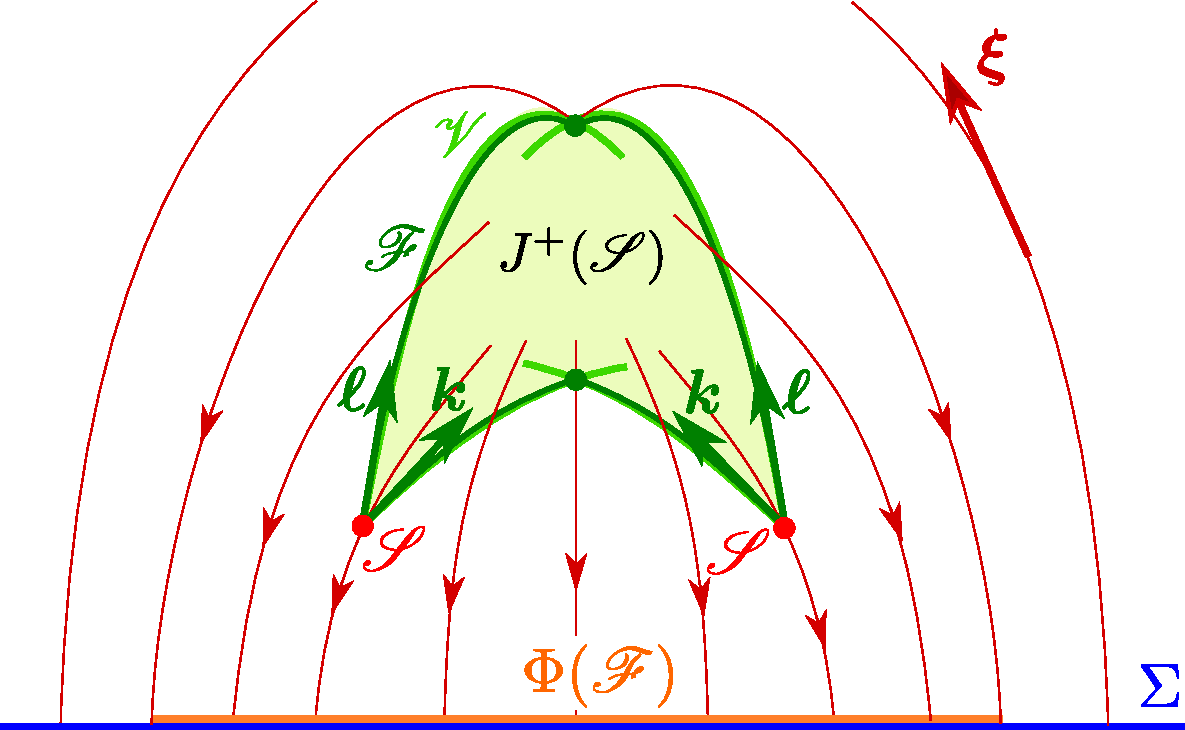
\includegraphics[width=0.7\textwidth]{loc_penrose_thm.pdf}}
\caption[]{\label{f:loc:penrose_thm} \footnotesize
2D spacetime diagram representing various quantities involved in the
proof of Penrose's singularity theorem (Property~\ref{p:loc:Penrose_sing_thm}):
the trapped surface $\Sp$ (the two red dots),
the two null directions $\wl$ and $\w{k}$ normal to $\Sp$,
the causal future of $\Sp$, $J^+(\Sp)$ (pale green region),
the boundary $\mathscr{F}$ (dark green curve)
of $J^+(\Sp)$, the compact space $\mathscr{V}$ containing $\mathscr{F}$ (light green)
and the image $\Phi(\mathscr{F})$ of $\mathscr{F}$ (orange segment) into
the Cauchy surface $\Sigma$ (blue line) by the topological embedding $\Phi$
constructed from the field lines (maroon lines) of a global timelike vector
$\w{\xi}$. The two dark green dots are crossover points, where null
geodesics leave $\mathscr{F}$ to the future.
The compact $(n-2)$-dimensional surface $\Sp$ appears as
two points for this 2D figure has to be thought as the cut by a vertical plane
of the 3D view of Fig.~\ref{f:neh:trapped_surf}, where $\Sp$ is drawn as
an horizontal circle.
}
\end{figure}



\begin{proof}
We shall prove the theorem by contradiction. Hence let us assume that all
inextendible null geodesics emerging orthogonally from $\Sp$ are future-complete. Let $\mathscr{F}$
be the boundary of the causal future of $\Sp$
(cf. Sec.~\ref{s:glo:causal_struct} and Fig.~\ref{f:loc:penrose_thm}): $\mathscr{F} := \partial J^+(\Sp)$.
$\mathscr{F}$ is an \emph{achronal boundary}\index{achronal!boundary}\index{boundary!achronal},
namely the boundary of the causal future or past of a given set.
As mentioned in Sec.~\ref{s:glo:properties_H} (Remark~\ref{r:glo:achronal_boundaries}),
the properties of an achronal boundary are the same as those established for a black hole event horizon
$\Hor = \partial J^-(\scri^+) \cap \M$ (Properties~\ref{p:glo:prop1} to \ref{p:glo:prop4}),
provided one changes \emph{future} to \emph{past} when appropriate.
It follows that $\mathscr{F}$ is an achronal $(n-1)$-dimensional topological manifold
(Properties~\ref{p:glo:prop1} and \ref{p:glo:prop2}) that is ruled by null geodesics,
called the \emph{generators}\index{generator!of an achronal boundary} of $\mathscr{F}$,
obeying the following properties:
when followed in the past direction, a generator never leaves $\mathscr{F}$ until it encounters $\Sp$
and there is a unique generator through each point of $\mathscr{F}$, except at special
points, named \emph{crossovers}\index{crossover point}, where the generators leave
$\mathscr{F}$ in the future direction,
i.e. are future-extended to null geodesics of $\M$ that do not belong
to $\mathscr{F}$ (Property~\ref{p:glo:prop3}). Note that two crossovers are shown in
Fig.~\ref{f:loc:penrose_thm}.

We actually need an additional property of $\mathscr{F}$,
which has not been established in Sec.~\ref{s:glo:properties_H}:
on  $\Sp$ (which is part of $\mathscr{F}$, cf. Sec.~\ref{s:glo:causal_struct}),
the generators of $\mathscr{F}$ are orthogonal to $\Sp$ (cf. e.g. Theorem~9.3.11
in Wald's textbook~\cite{Wald84}). They therefore start from $\Sp$ along
the two null directions $\wl$ and $\w{k}$ normal to $\Sp$ (cf. Fig.~\ref{f:loc:penrose_thm}). Let us denote by $\Li$ the null
generators along $\wl$ and by $\lambda$ the affine parameter of $\Li$
such that, on $\Sp$, $\lambda = 0$ and $\left. \D\w{x}/\D\lambda\right| _\Li = \wl$. We shall use
the latter relation to extend the definition of $\wl$ along $\Li$
away from $\Sp$. Similarly, let us denote by $\bar{\Li}$ the null
generators along $\w{k}$ and by $\bar\lambda$ the affine parameter of $\bar{\Li}$
such that $\bar\lambda = 0$ on $\Sp$ and
$\left. \D\w{x}/\D\bar\lambda \right| _{\bar{\Li}}= \w{k}$.
By hypothesis, $\Li$ and $\bar{\Li}$ are future-complete.
Since $\Sp$ is a trapped surface, $\theta_0 := \left. \theta_{(\wl)} \right| _{\Sp} < 0$
and $\bar\theta_0 := \left. \theta_{(\w{k})} \right|_{\Sp}<0$.
Then, thanks to the
null Raychaudhuri equation\index{null!Raychaudhuri equation}\index{Raychaudhuri!null --  equation}
(\ref{e:def:null_Raychaud_Ricci}),
the null energy condition $\w{R}(\wl,\wl) \geq 0$ implies that there exists $\lambda_* \in (0, (n-2)/|\theta_0|]$
such that $\theta_{(\wl)} \to -\infty$ for $\lambda\to \lambda_*$ along $\Li$.
The reasoning is exactly the same at that used in the proof of
Property~\ref{p:evo:positive_expansion} and we shall
not repeat it here. The point $\lambda=\lambda_*$ on $\Li$ is a caustic point,
where all nearby geodesics starting from $\Sp$ along $\wl$ converge.
Given the properties of $\mathscr{F}$, we conclude that for $\lambda > \lambda_*$, $\Li$
ceases to a be null generator of $\mathscr{F}$, i.e.
$\Li_{\lambda > \lambda_*} \not\in \mathscr{F}$.
Similarly, along $\bar{\Li}$,
$\theta_{(\w{k})} \to -\infty$ for $\bar\lambda\to \bar\lambda_*$
with $\bar\lambda_* \in (0, (n-2)/|\bar\theta_0|]$, so that
$\bar{\Li}_{\bar\lambda > \bar\lambda_*} \not\in \mathscr{F}$.
Let
\[
    \lambda_{\rm max} := \sup_{p\in\Sp} \left(  \frac{n-2}{|\theta_{(\wl)} (p)|} \right)
    \qand
    \bar\lambda_{\rm max} := \sup_{p\in\Sp} \left(  \frac{n-2}{|\bar\theta_{(\w{k})}(p)|} \right)    .
\]
Since $\Sp$ is compact, $\lambda_{\rm max}$ and $\bar\lambda_{\rm max}$ are finite.
Let us then consider the map $f: \Sp \times [0,\lambda_{\rm max}] \to \M$,
$(p,\lambda) \mapsto q$, where $q$ is the point of affine parameter $\lambda$
on the null geodesic of the $\Li$-family through $p$.
Since all the $\Li$ geodesics are assumed to be future-complete, $f$ is well defined.
Moreover, $f$ is clearly continuous. Then, given that
$\Sp \times [0,\lambda_{\rm max}]$ is a compact set, the image set
$f(\Sp \times [0,\lambda_{\rm max}])$ is necessarily compact. Similarly, the image set
$\bar{f}(\Sp \times [0,\bar\lambda_{\rm max}])$ is compact, where
$\bar{f}: \Sp \times [0,\bar\lambda_{\rm max}] \to \M$, $(p,\lambda) \mapsto \bar{q}$ --- the point of affine parameter $\bar\lambda$
on the null geodesic of the $\bar{\Li}$-family through $p$.
The set
\[
    \mathscr{V} := f\left(\Sp \times [0,\lambda_{\rm max}]\right)
        \cup \bar{f}\left(\Sp \times [0,\bar\lambda_{\rm max}]\right)
\]
is then a compact subset of $\M$, as the union of two such sets. By construction, for each $p\in\Sp$, the
point $q = f(p,\lambda_{\rm max})$ (resp. $\bar{q} = f(p,\lambda_{\rm max})$)
lies beyond the caustic point on the geodesic $\Li$ (resp. $\bar{\Li}$)
through $p$. It follows that $\mathscr{F} \subset \mathscr{V}$ (cf. Fig.~\ref{f:loc:penrose_thm}).
Given that $\mathscr{F}$
is closed, being a topological boundary ($\mathscr{F} := \partial J^+(\Sp)$),
and $\mathscr{V}$ is compact, we conclude that $\mathscr{F}$ is compact.

Because $(\M,\w{g})$ is time-orientable, there exists a nonvanishing
timelike vector field $\w{\xi}$ on $\M$. The field lines of $\w{\xi}$
form a congruence of timelike curves $\mathscr{C}$, each of them intersecting
$\Sigma$ in a single point, for $\Sigma$ is a Cauchy surface.
We may then define a map $\Phi: \mathscr{F} \to \Sigma$,
$p \mapsto \mathscr{C}_p \cap \Sigma$, where $\mathscr{C}_p$ is the unique
timelike curve of the $\mathscr{C}$ congruence through $p$.
The map $\Phi$ is clearly continuous. Moreover, it is injective given that
$\mathscr{F}$ is achronal (if a point $q\in\Sigma$ was the image of two distincts
points $p$ and $p'$ of $\mathscr{F}$, this would mean that $p$ and $p'$
are connected by a timelike curve, namely a segment of $\mathscr{C}_p$).
Now, there cannot be any injective continuous map from a
compact manifold (without boundary) (here $\mathscr{F}$)
into a non-compact manifold of the same dimension (here $\Sigma$). For instance,
there is no injective continuous map from the sphere $\mathbb{S}^2$ into
the plane $\R^2$. To show this impossibility in the present case, and hence
to reach the sought contradiction, let us invoke a
standard topology theorem (see e.g. Lemma~4.50
in Lee's textbook~\cite{Lee11}), according to which an injective continuous map
from a compact space to a Hausdorff space
is a topological embedding, i.e. a homeomorphism onto its image. This theorem applies here
since $\Sigma$ is Hausdorff, being a manifold (cf. Sec.~\ref{s:bas:def_manif}).
Hence $\Phi(\mathscr{F})$ is homeomorphic to $\mathscr{F}$.
$\Phi(\mathscr{F})$ is therefore a compact subset of $\Sigma$.
Another standard result of topology (see e.g. Proposition 4.36b in Lee's textbook~\cite{Lee11})
states that a compact subset of a Hausdorff space is closed. Hence $\Phi(\mathscr{F})$
is a closed subset of $\Sigma$.
On the other side, since $\mathscr{F}$ is a $(n-1)$-dimensional topological manifold,
each point of $\mathscr{F}$
has a neighborhood homeomorphic to an open subset of $\R^{n-1}$. The same thing holds then for
$\Phi(\mathscr{F})$. Since $\Sigma$ is a $(n-1)$-dimensional manifold, it follows that
$\Phi(\mathscr{F})$ is an open subset of $\Sigma$. Hence $\Phi(\mathscr{F})$ is both open
and closed in $\Sigma$. Given that $\Sigma$ is connected, being a Cauchy surface in
a connected spacetime, this implies that
$\Phi(\mathscr{F}) = \Sigma$. Here we reach a contradiction because $\Sigma$
is assumed non-compact. The proposition that all
null geodesics emerging orthogonally from $\Sp$ are future-complete is thus false.
\end{proof}

\subsection{Hawking \& Penrose's singularity theorem}


%%%%%%%%%%%%%%%%%%%%%%%%%%%%%%%%%%%%%%%%%%%%%%%%%%%%%%%%%%%%%%%%%%%%%%%%%%%%%%%

\section{Trapping horizons}


